\section{\Multidispatch{} Linearizability}
\label{sec:mdl}

In this section, we first define \multidispatch{} linearizability.
We then show how applications built atop an \MDL{} system appear
to behave identically (as far as users can tell) to the same application interacting
with a comparable \SDL{} system. Finally, we discuss existing implementations
of \MDL{} for single-shard systems and why they do not trivially extend to more
shards.

We leverage the formalism used in Helt et al.~\cite{helt2021rss}.

\subsection{Users, Applications, \& Executions}
\label{sec:mdl:applications}

We model a distributed \textit{application} as a collection of $n$
\textit{processes}. Processes are state machines~\cite{lynch1987ioa,lynch1996da}
that implement application logic by performing local computation, exchanging
messages, and invoking operations on systems.

An application's processes define a prefix-closed set of \textit{executions},
which are sequences $s_0,\pi_1,s_1,\ldots$ of alternating \textit{states} and
\textit{actions}, starting and ending with a state. An application state
contains the state of each process---it is an $n$-length vector of process
states. As part of a process's state, we assume it has access to a local
clock, which it can use to set local timers, but the clock makes no guarantees
about its drift or skew relative to those at other processes.

Each action is a step taken by exactly one process and is one of three types:
\textit{internal}, \textit{input}, or \textit{output}. Internal actions model
local computation. Processes use input and output actions to interact with other
processes (e.g., receiving and replying to a remote procedure call) and their
environment (e.g., responding to a user gesture). As we will describe in the
following section, a subset of the input and output actions are
\textit{invocations} and \textit{responses}, respectively, which are used to
interact with systems.

Processes can also exchange messages with one another via unidirectional
channels. To send a message to process $P_j$, $P_i$ uses two actions: first,
$P_i$ uses an output action $\sendto_{ij}(m)$ and later, an input action
$\sent_{ij}$ occurs, indicating $m$'s transmission on the network. Similarly, to receive a
message from $P_i$, $P_j$ first uses an output action $\request_{ij}$ and later,
an input action $\receive_{ij}(m)$ occurs, indicating the receipt of $m$.

Given an execution $\alpha$, we will often refer to an individual process's
\textit{sub-execution}, denoted $\alpha|P_i$. $\alpha|P_i$ comprises
only $P_i$'s actions and the $i$th component of each state in $\alpha$.

\noindentparagraph{Well-formed.} An execution is \textit{well-formed} if it
satisfies the following: (1) Messages are sent before they are received; (2) A
process has at most one (total) outstanding invocation (at a system)
or $\request_{ij}$ (at a channel); and (3) Processes do not take output steps while
waiting for a response from a system. We henceforth only consider well-formed executions.

TODO: Update definition of well-formed.
% A \textit{process sub-history} $H|P$ is the subsequence of all invocations and responses
% in $H$ invoked or received by the application process $P$. To define \MDL{}, we relax the
% assumption made by Herlihy et al.~\cite{herlihy1990linearizability} that process sub-histories
% (i.e., their interactions with the system) are sequential. Instead, we say a history $H$
% is \textit{well-formed} if the following hold for each process sub-history $H|P$:
% (1) $H|P$ starts with an invocation, and (2) for each operation $o$, if $\res(o)$ is in $H$,
% it follows (not necessarily immediately) $\inv(o)$. We consider only well-formed histories.

TODO: Add users.

TODO: Define $||$.
% Given a history $H$, $H||P$ is a \textit{sequentialization} of $H|P$. $H||P$ is
% found by, for each complete operation $o$ in $H|P$, shifting $\res(o)$ left (earlier) in $H|P$
% until it immediately follows $\inv(o)$. Note that if $H|P$ is sequential, then $H|P = H||P$.

\subsection{Systems}
\label{sec:mdl:systems}

Databases, message queues, and other back-end \textit{systems} that application
processes interact with are defined by their \textit{operations} and a
\textit{specification}~\cite{herlihy1990linearizability,lynch1996da}. An
\textit{operation} comprises pairs of \textit{invocations}, specifying the
operations and their arguments, and matching \textit{responses}, containing
return values. The specification is a prefix-closed set of sequences of
invocation-response pairs defining the system's correct behavior in the absence
of concurrency. A sequence $S$ in specification $\spec$ defines a total order
over its operations, denoted $<_S$.

\subsection{Definition}
\label{sec:mdl:def}

We are now ready to define two (last) preliminaries and then our new consistency model.

\noindentparagraph{Complete operations.} Given an execution $\alpha$, we say an
operation is \textit{complete} if its invocation has a matching response in
$\alpha$. We denote $\complete(\alpha)$ as the maximal subsequence of $\alpha$
comprising only complete operations~\cite{herlihy1990linearizability}.

\noindentparagraph{Real-time order.} Two actions in an execution $\alpha$ are
ordered in real
time~\cite{herlihy1990linearizability}, denoted
$\pi_1 \rt_\alpha \pi_2$, if and only if $\pi_1$ is a response, $\pi_2$ is an
invocation, and $\pi_1$ precedes $\pi_2$ in $\alpha$.

\noindentparagraph{\Multidispatch{} Linearizability.} Let $\mathcal{O}$ be the
set of all operations. An execution $\alpha_1$ satisfies \textit{\MDL{}} if it
can be extended to $\alpha_2$ by adding zero or more responses such that there
exists a sequence $S \in \spec$ where (1) for all $P$,
$S|P = \complete(\alpha_2)||P$; and (2) for all pairs of operations
$o_1,o_2 \in \mathcal{O}$, $o_1 \rt_{\alpha_1} o_2 \implies o_1 <_S o_2$.

\subsubsection{Suffix-Closed Failures}
\label{sec:mdl:def:failures}

\MDL{}'s definition has an important implication for system designers.
In systems where operations can fail (even temporarily before being retried), the effects
of an operation cannot be exposed to other processes until all of its predecessors are
guaranteed to succeed. Doing so would violate the intuitively correct behavior of most
systems, and formally, this would result in $S|P \neq \complete(\alpha_2)||P$ for all legal
sequential histories $S \in \spec$. We refer to this property as
\textit{suffix-closed failure semantics}.

In an \MDL{} system, suffix-closed failures must be guaranteed even in the
face of concurrent operations from the same process, which in practice may to
objects on different shards. As we will see in Section~\ref{sec:mdl:zookeeper},
guaranteeing suffix-closed failures is one way in which existing systems fail
to correctly implement \multidispatch{} linearizability.  

\subsection{External Equivalence}
\label{sec:mdl:equivalence}

\noindentparagraph{Equivalence.} Two executions $\alpha$ and $\beta$ are
\textit{equivalent} if for all $P_i$, $\alpha|P_i = \beta|P_i$. Intuitively,
equivalent executions are indistinguishable to the processes.

\subsection{\MDL{} Beyond One Shard}
\label{sec:mdl:zookeeper}

In this section, we discuss Zookeeper and its implementation of \SDL{}.
We also show how such an approach does not extend to multiple shards.

\begin{figure}[!htb]
    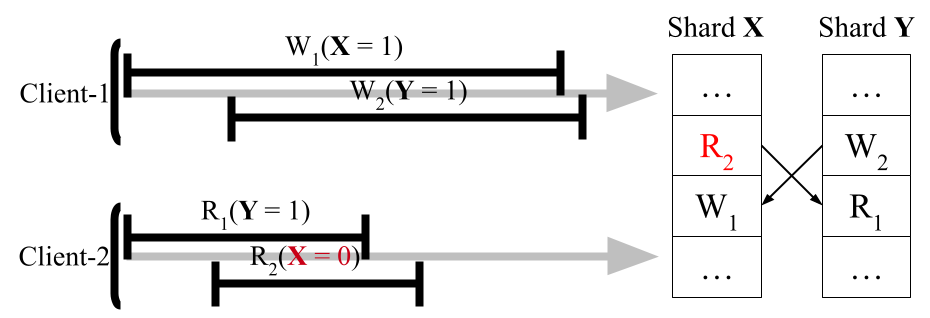
\includegraphics[scale=.45]{somet.png}
    \caption{Example execution where two concurrent clients each submit 2 concurrent requests. Assume keys \textbf{X} and \textbf{Y} are at different shards. It is possible that $R_2$ arrives before $W_1$ at shard \textbf{X}, and $W_2$ arrives before $R_1$ at shard \textbf{Y}. Since clients expect their concurrent requests to take affect in invocation order, if $R_1$ returns 1, then $W_1$ must have taken affect before $R_1$, so $R_2$ should necessarily return a value of 1.}
    \label{fig:concurrentbatches}
\end{figure}

For the single-shard setting, existing protocols come close to providing \MDL{}. A simple mechanism, such as per-client sequence numbers, can provide enough information for a shard leader to support invocation order for multiple requests from a single client. Such a solution does not suffice in the multi-shard setting, however, as shown in figure ~\ref{fig:concurrentbatches}. Linearizability is a local property, thus a single-shard protocol correctly scales to multiple shards. \MDL{}, however, is not a local property due to the possible interleaving of sets of concurrent requests across concurrent clients.
% Jeff: I don't think we want (or need) to make the claim below.
% This requires an \MDL{} protocol to use inter-shard communication in order to guarantee a safe total ordering that reflects issue order.

Sequence numbers are assigned at the client library 
and increase monotonically per shard. For example, a client issuing two requests for the first time to different keys that are on different shards will issue two requests both with sequence number 0. The shard leaders can then easily detect when a client's request
has arrived out of order and can buffer it until the necessary predecessor requests intended for the same shard arrive.
